\subsubsection{\atlas{Prospects for $Z'$ searches at HL-LHC and HE-LHC}}
\contributors{M. Wielers, G. Lee, M. Marjanovic et al., ATLAS}\rt{There are comments to address.}
%{\bf Author(s): M. Wielers, G. Lee, M. Marjanovic et al., ATLAS}

%Searches for Z' (SSM and other models) are performed considering the dilepton (ee, mumu) final state events. Prospects for discovery and exclusion considering 13, 14 and 15 TeV datasets as well as HE-LHC are presented. 

The sensitivity to narrow $Z^\prime$ bosons decaying into the $e^+e^-$ or $\mu^+\mu^-$ final state
is studied for $pp$ collisions at several \com energies: $\sqrt{s} = 13$, 14, and 15~TeV
with 3000~fb$^{-1}$,
as well as $\sqrt{s} = 27$~TeV with 15~ab$^{-1}$.
The latter is only studied in the $e^+e^-$ channel since the work presented here is based on the latest
layout of the upgraded ATLAS detector for the HL-LHC which is not optimized for extremely high
muon momentum measurements.
The study supersedes that from \citeref{ATLAS:prospectives_zprime} since it uses the latest detector
layout, higher pileup conditions, and updated signal cross sections. since the values in
\citeref{ATLAS:prospectives_zprime} were found to be too high.

The projection study relies on MC simulation for the signal based on \pythia{8}~\cite{pythia8}, the \sloppy\mbox{\textsc{NNPDF23LO}} PDF set~\cite{Ball:2012cx}, and the A14 set of tuned parameters~\cite{ATL-PHYS-PUB-2014-021} for the parton shower, hadronisation, and the underlying event. The dominant Drell-Yan background source is generated with \powhegbox~\cite{powheg1,powheg2} and the \textsc{CTEQ6L1} PDF set~\cite{Pumplin:2002vw} interfaced with \pythia{8} for the parton shower, hadronisation and the underlying event using the \textsc{AZNLO} set of tuned parameters~\cite{AZNLO:2014}.

The event selection proceeds in a way similar to the analysis of the 13~TeV data with
36.1~fb$^{-1}$~\cite{Aaboud:2017buh}.
Events must pass either the single-electron trigger requirements with $p_\mathrm{T} > 22$~GeV and
$|\eta| < 2.5$ or the single-muon trigger requirements with $p_\mathrm{T} > 20$~GeV and $|\eta| < 2.65$.
Triggered events are further required to contain exactly two electrons with $p_\mathrm{T} > 25$~GeV
and $|\eta|<2.47$ (excluding the barrel-endcap calorimeter transition region $1.37 < |\eta| < 1.52$)
or two muons with $p_\mathrm{T} > 25$~GeV and $|\eta| < 2.65$.
The electrons and muons have to satisfy the \textit{tight} and
\textit{high-$p_\mathrm{T}$}~identification requirements, respectively.
The corresponding signal acceptance times efficiency reaches a maximum of 78\% (55\%)
for $Z^\prime$ masses between 5 and 11~TeV in the dielectron (dimuon) channel.
These values do not change appreciably at the different \com energies examined here.
Invariant mass distributions of the reconstructed dielectron and dimuon candidates are shown
in \fig{fig:ATLAS_Zprimell_mll} for the $Z^\prime_\mathrm{SSM}$ signal and the dominant
Drell-Yan background.
Background from diboson ($WW$, $WZ$, $ZZ$) and top-quark production is not considered as their
contribution to the overall SM background is negligible for dilepton invariant masses ($m_{\ell\ell}$)
exceeding 2~TeV. This background is more pronounced at lower masses and was found to amount to
around 10\% (20\%) of the total background for an invariant mass of 1~TeV (300~GeV),
see \citeref{Aaboud:2017buh}.
In the dielectron channel, additional background arises from $W+$jets and multijet events
in which at most one real electron is produced and one or more jets satisfy the electron selection
criteria. While this background is negligible in the dimuon channel, it amounts to approximately
15\% of the total background for $m_{\ell\ell} > 1$~TeV~\cite{Aaboud:2017buh} in the dielectron channel.
This source of background is neglected in the analysis below but accounted for in the systematic
uncertainties.
\begin{figure}[tbp]
\centering
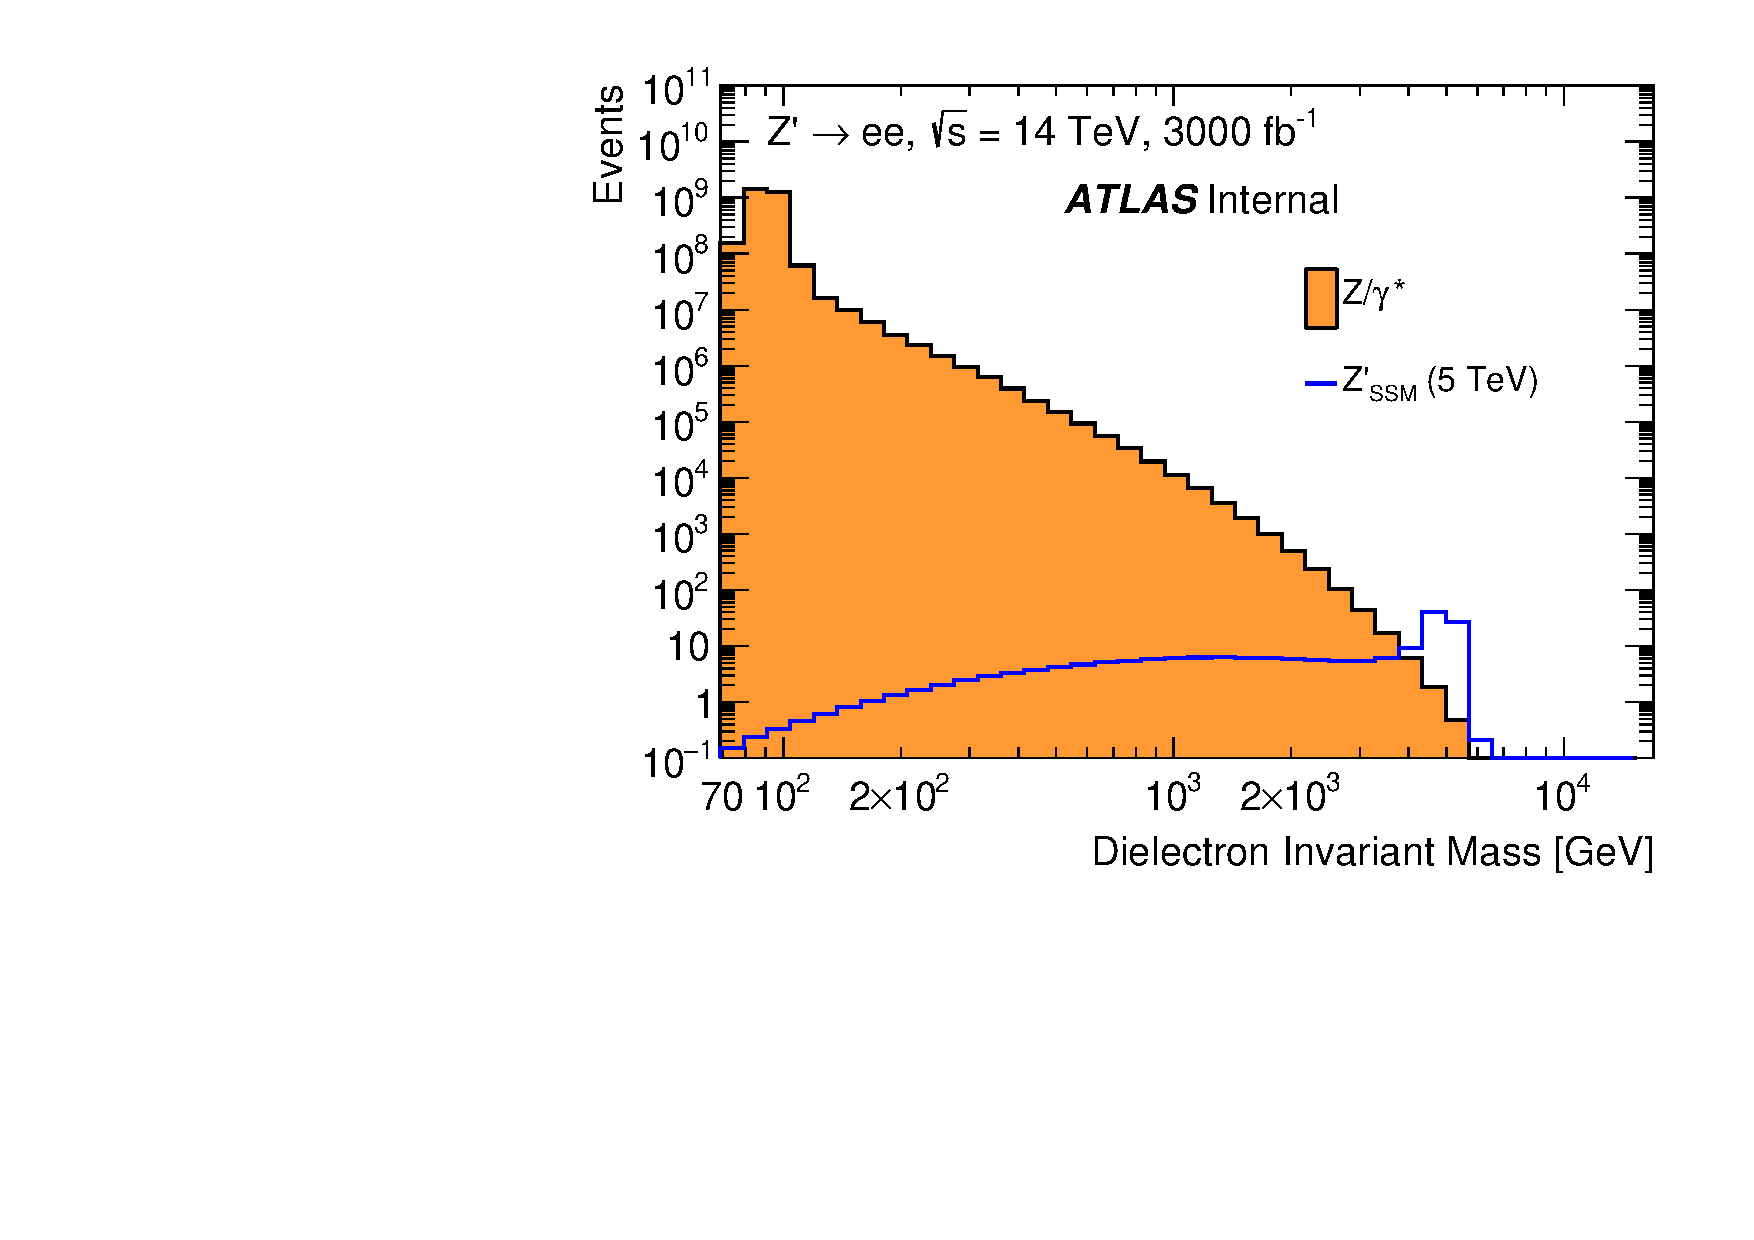
\includegraphics[width=0.325\columnwidth]{./section7OtherSignatures/img/Zee_Mll_5000M_smear.pdf}
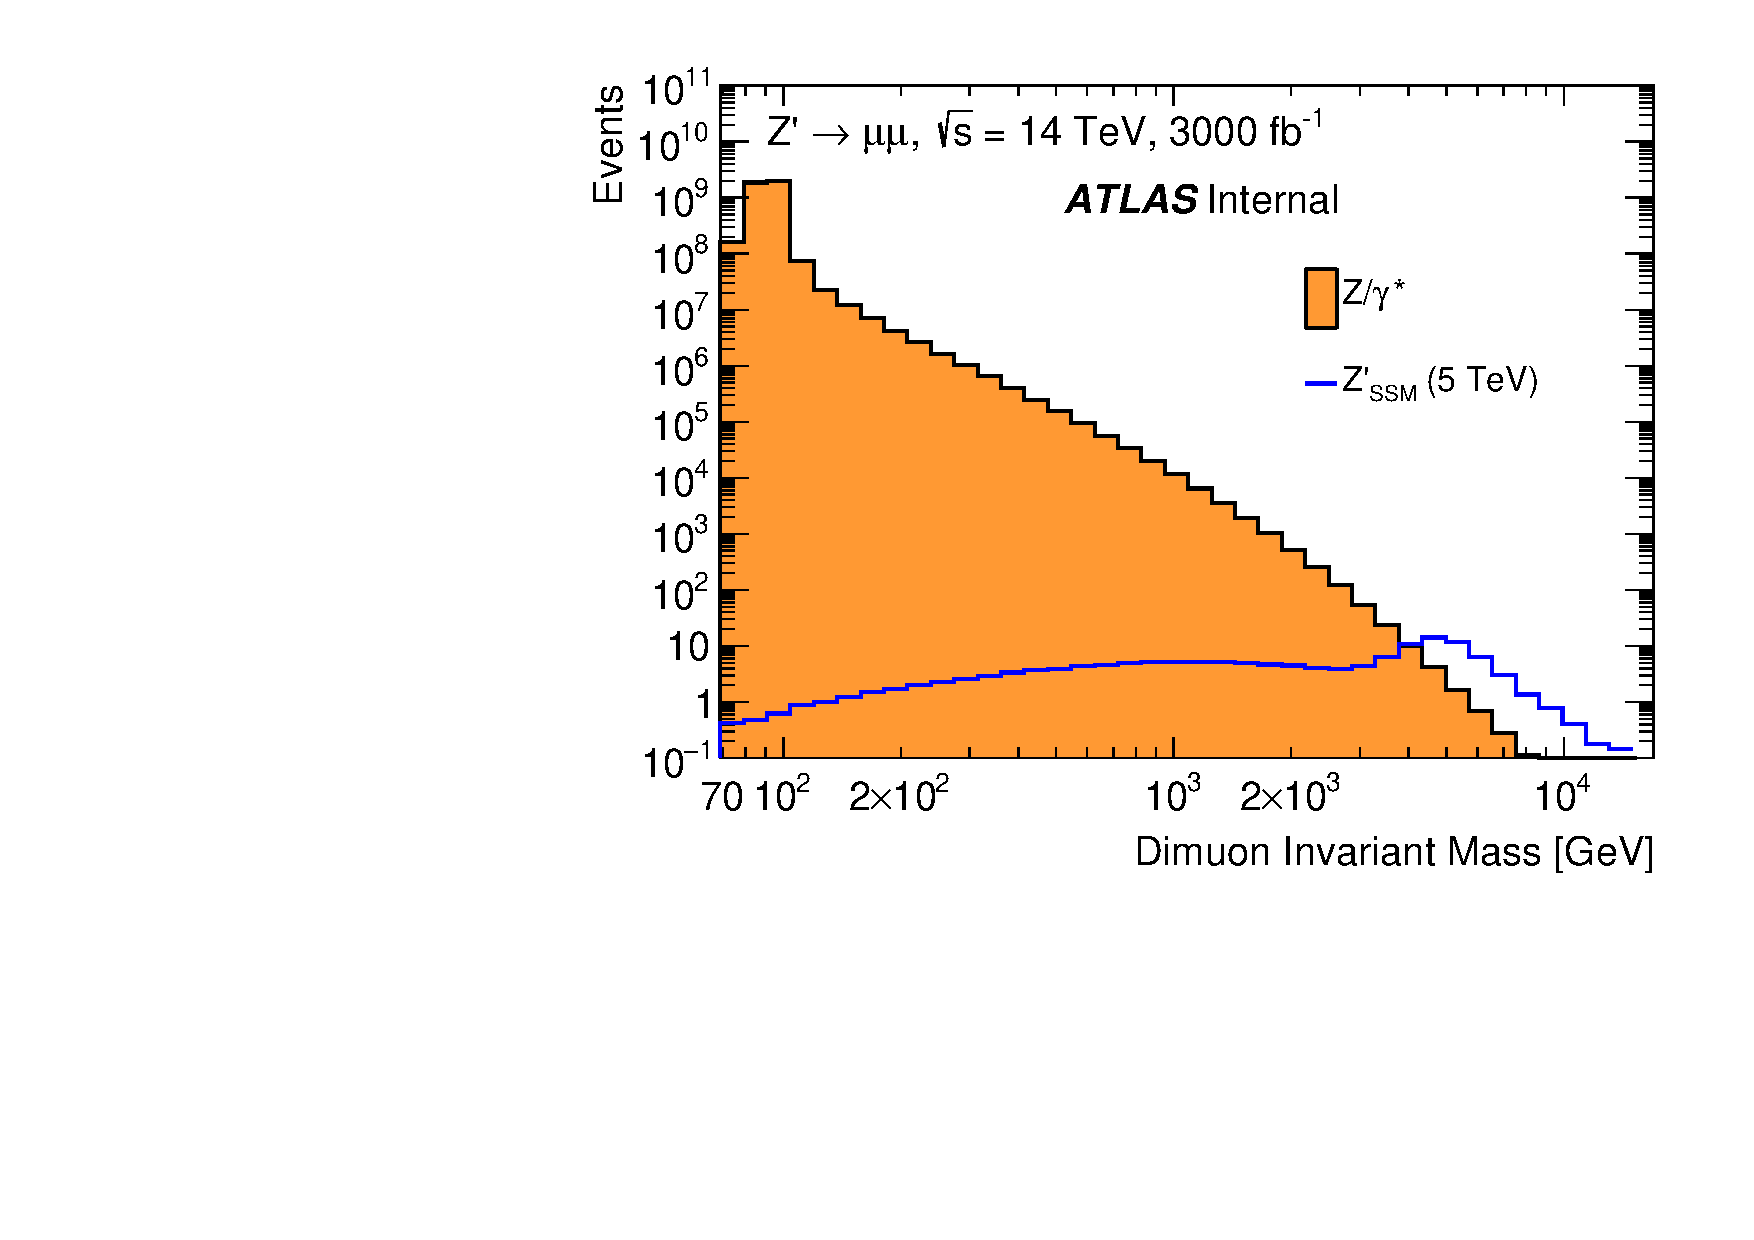
\includegraphics[width=0.325\columnwidth]{./section7OtherSignatures/img/Zmumu_Mll_5000M_smear.pdf}
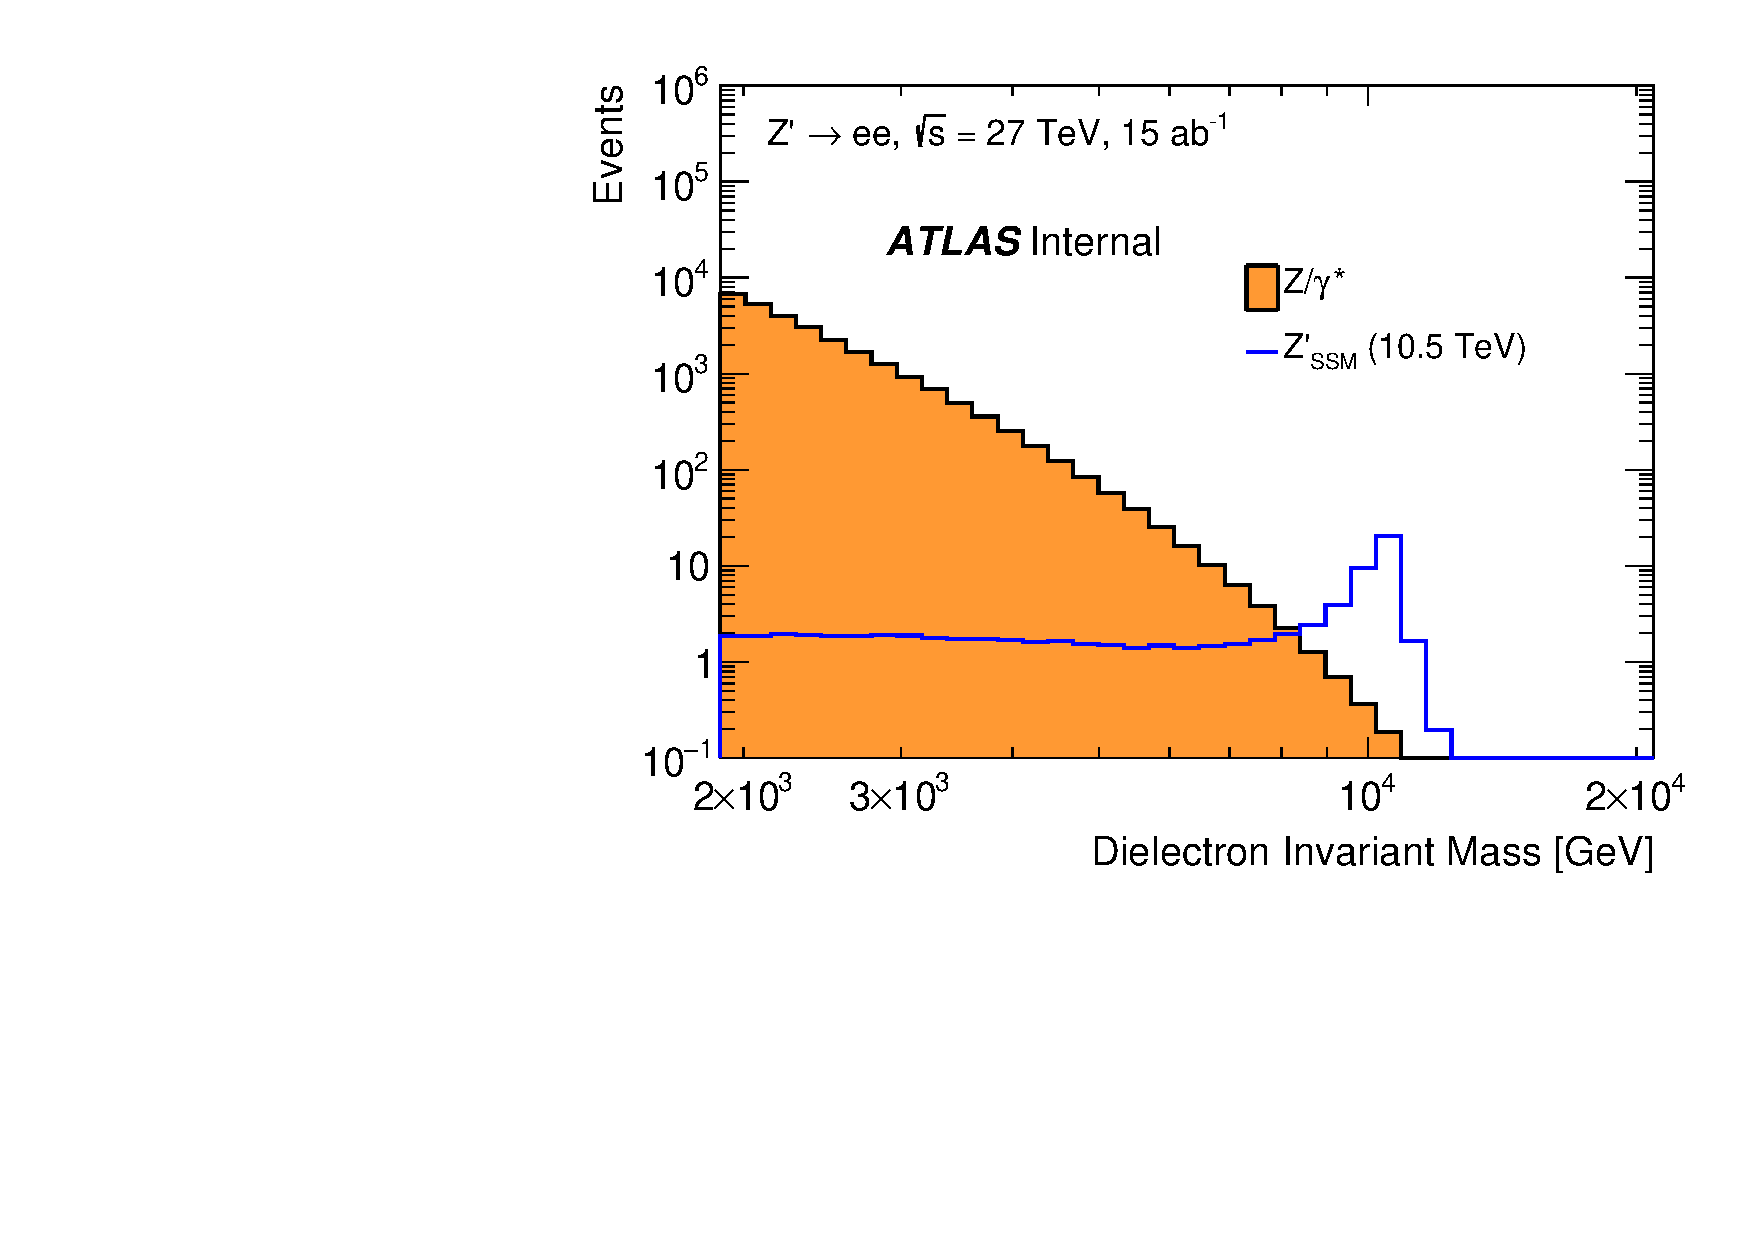
\includegraphics[width=0.325\columnwidth]{./section7OtherSignatures/img/Zee_Mll_10500M_smear.pdf}
  \caption{
    Invariant mass distributions for events satisfying all selection criteria in the dielectron and dimuon channels at $\sqrt{s}=14$~TeV and in the dielectron channel at $\sqrt{s}=27$~TeV.
    Distributions of the Drell-Yan background and SSM $Z^\prime$ signal with a mass of 5.0 (10.5) TeV
    are shown for $\sqrt{s} = 14$ (27) TeV.
}
\label{fig:ATLAS_Zprimell_mll}
\end{figure}
%
The differences in the shape of the reconstructed $Z^\prime$ mass distributions in the dielectron and dimuon
channels arise from differences in momentum resolution for electron and muon reconstruction.
The differences in the shape of the dielectron mass distributions at $\sqrt{s}=14$~TeV and 27~TeV
arise from differences in the rapidity distributions.

The experimental and theoretical uncertainties assumed in this analysis are estimated from the
Run~2 results~\cite{Aaboud:2017buh} but scaled down to account for the increased statistical
precision available at the HL-LHC following the recommendations in \citeref{atlasperf}.
Only the largest sources of uncertainties are considered. As the uncertainties vary
with $m_{\ell\ell}$, the uncertainties are expressed relative to the value of $m_{\ell\ell}$ given in TeV.

The experimental systematic uncertainties due to the reconstruction, identification, and isolation
of electrons are negligible while those for muons add up to approximately $2.5\% \times m_{\ell\ell}$~[TeV]. 
Systematic uncertainties due to the energy resolution and scale are set to $1.5\% \times m_{\ell\ell}$~[TeV]. 
The uncertainties due to the resolution and reconstruction of the leptons are added in quadrature
to the dominant sources of theoretical uncertainty due to the PDFs. The uncertainties due to the choice of PDF set are taken to be 
$2.5\% \times m_{\ell\ell}$~[TeV] and the uncertainties in the parameters of the nominal PDF set are assumed
to be $5\% \times m_{\ell\ell}$~[TeV]. 
Overall these uncertainties add up to $~6.5\% \times m_{\ell\ell}$~[TeV].
As the search looks for an excess in the high $m_{\ell\ell}$ tail, the sensitivity is primarily
limited by the statistical uncertainties.

The statistical analysis relies on the Bayesian approach~\cite{Caldwell:2008fw}
used in~\citeref{Aaboud:2017buh}.
The same statistical model implementation is used in the following for both the calculation of the exclusion
limits and the discovery reach, the latter being based on a profile likelihood ratio test assuming
an asymptotic test statistic distribution.
In the absence of a signal, 95\%~\cl upper limits are placed on the production cross section of
a $Z^\prime$ boson times its branching fraction $\sigma \times \cal{B}$ to a single lepton generation,
assuming lepton universality.
These limits are extracted using $Z^\prime$ templates binned in $m_{\ell\ell}$ for a series 
of $Z^\prime$ masses in the range between 3.5~TeV and 11.5~TeV.
The interpretation of results is performed in the context of the Sequential Standard Model (SSM) and the $E_6~\psi$ model
as shown in \fig{fig:ATLAS_Zpll_limits} for the latter model.\rt{SSM does not appear in final plot. Why?}\rt{My usual concern. When the Z' starts getting a large off-shell contribution to its production CS, then the bound is not anymore on $\sigma\times\cal{B}$. The bound is on $\sigma(pp\to l\nu)$. A limit on $\sigma\times\cal{B}$ cannot grow at high masses, it should be constant.}
\begin{figure}[htbp]
\centering
%\subfigure[]{\includegraphics[width=0.48\columnwidth]{figures/Limit_xsec_zprime_Psi_ee_Sys_3000ifb_14TeV.eps} }
%\subfigure[]{\includegraphics[width=0.48\columnwidth]{figures/Limit_xsec_zprime_Psi_mm_Sys_3000ifb_14TeV.eps} }
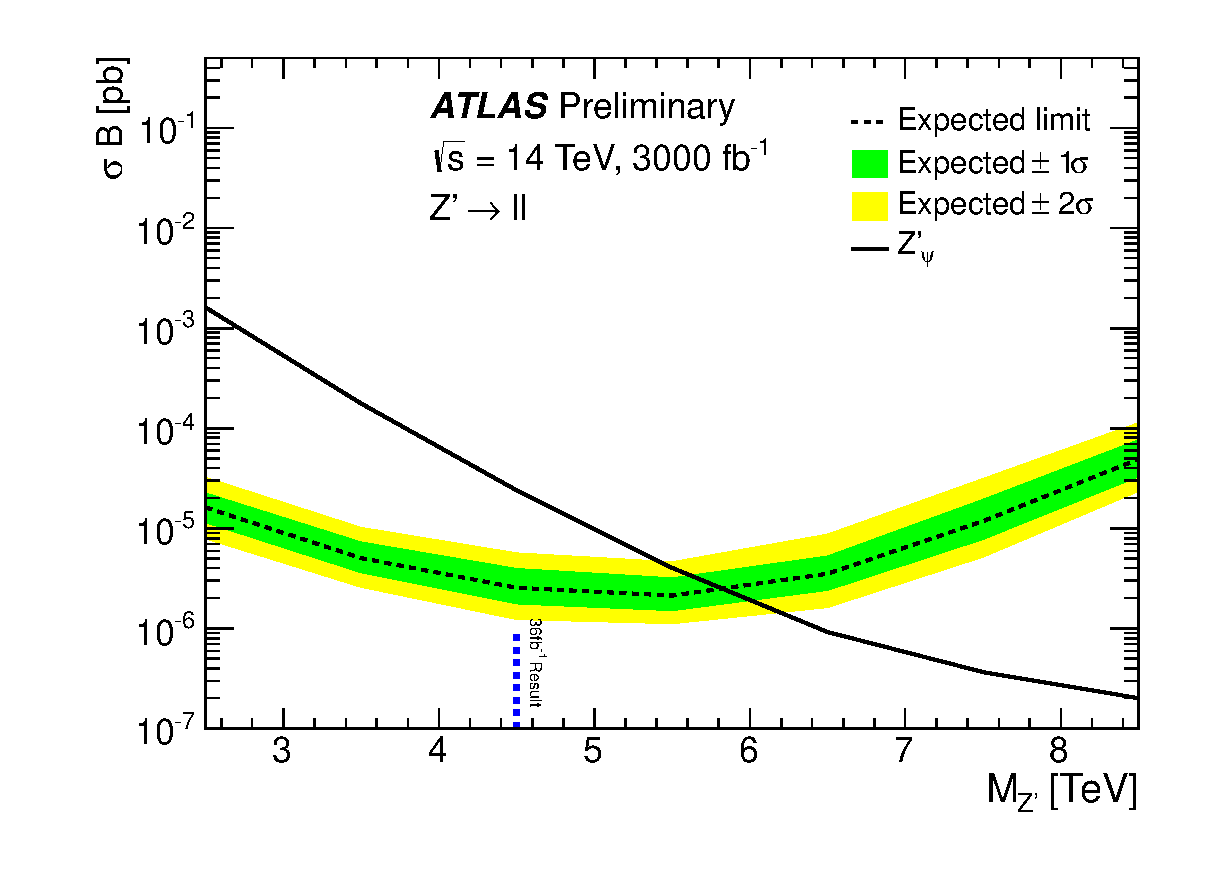
\includegraphics[width=0.48\columnwidth]{./section7OtherSignatures/img/Limit_xsec_zprime_Psi_comb_Sys_3000ifb_14TeV.eps}
  \caption{
    Expected (dashed black line) upper limit on cross-section times branching fraction $\sigma \times \cal{B}$  as a function of the
    $Z^\prime$ boson mass in the combined dielectron and dimuon channels for $\sqrt{s} = 14$~TeV collisions
    and an integrated luminosity value of 3000~fb$^{-1}$. The $1\sigma$ (green) and $2\sigma$ (yellow)
    expected limit bands are also shown. The predicted $\sigma \times \cal{B}$ for $Z^\prime_\psi$ production
    is shown as a black line. The blue marker shows the current limit obtained with the Run~2 analysis
    based on 36~fb$^{-1}$ of data.
}
  \label{fig:ATLAS_Zpll_limits}
\end{figure}
%
Lower mass limits and the discovery reach for the different models and $\sqrt{s}$ values
at the HL-LHC are summarised in \tabb{tab:ATLAS_zplllimits}. %and visualised in Figure~\ref{fig:zplllimits}.
The projected exclusion limits extend the current $Z^\prime_\mathrm{SSM}$ ($Z^\prime_\psi$) lower mass limit of 4.5 (3.8)~TeV
obtained using 36.1~fb$^{-1}$ of data taken at $\sqrt{s} = 13$~TeV to 6.7 (6.1)~TeV.
Higher limits are obtained in the dielectron channel due to the superior energy resolution of
the calorimeter as compared with the momentum resolution for muons in the muon spectrometer.
Assuming similar detector performance at the LHC and HL-LHC, a corresponding lower mass limit of 5.4 (4.8)~TeV are expected with 300~fb$^{-1}$ at the end of Run~3. 
The 95\%~\cl limits and discovery reach are close due to the absence of background at very high $m_{\ell\ell}$.
Compared to the results presented in \citeref{CERN-LHCC-2017-018} the discovery reach reported
here is higher due to a change in how the reach is calculated. The analysis described here
is based on the shape of the signal and background $m_{\ell\ell}$ distributions while the
$5\sigma$ significance was calculated in a mass range between $m(Z^\prime)/2$ to infinity in
\citeref{CERN-LHCC-2017-018}.
\begin{table}[!tbp]
  \caption{Expected 95\%~\cl lower limit on the $Z^\prime$ mass in TeV in the dielectron and dimuon channels and their combination for two benchmark $Z^\prime$ models for different centre of mass energies assuming 3000~fb$^{-1}$ of data to be taken at the HL-LHC. In addition, the discovery reach for finding such new heavy particles is shown.}
  \centering
  \begin{tabular}{c|cc|cc|cc}
    \hline
    \hline
    &  \multicolumn{2}{c|}{$\sqrt{s} = 13$~TeV} &  \multicolumn{2}{c|}{$\sqrt{s} = 14$~TeV} &  \multicolumn{2}{c}{$\sqrt{s} = 15$~TeV} \\
    Decay     &  Exclusion & Discovery&  Exclusion& Discovery &  Exclusion & Discovery \\
    \hline
    $Z^\prime_\mathrm{SSM} \to ee$  & 6.0 TeV& 5.9 TeV & 6.4 TeV& 6.3 TeV & 6.7 TeV& 6.6 TeV\\
    $Z^\prime_\mathrm{SSM} \to \mu\mu$& 5.5 TeV& 5.4 TeV& 5.8 TeV& 5.7 TeV& 6.0 TeV& 5.9 TeV\\ \hline
    $Z^\prime_\mathrm{SSM} \to \ell\ell$  & 6.1 TeV& 6.1 TeV&6.5 TeV& 6.4 TeV& 6.7 TeV& 6.7 TeV\\
    \hline
    \hline
    $Z^\prime_\psi \to ee$  & 5.3 TeV& 5.3 TeV& 5.7 TeV& 5.6 TeV & 6.1 TeV& 6.0 TeV\\
    $Z^\prime_\psi \to \mu\mu$& 4.9 TeV & 4.6 TeV& 5.2 TeV& 5.0 TeV& 5.5 TeV& 5.2 TeV\\ \hline
    $Z^\prime_\psi \to \ell\ell$  & 5.4 TeV& 5.4 TeV&5.8 TeV& 5.7 TeV& 6.1 TeV& 6.1 TeV\\
    \hline
    \hline
    
  \end{tabular}
  \label{tab:ATLAS_zplllimits}
\end{table}

The discovery reach and lower exclusion limits at 95\%~\cl in mass are also calculated for a detector at the HE-LHC in the dielectron channel. This is done assuming the same physics performance as for the ATLAS detector at the HL-LHC.
The exclusion limits and the discovery reach are summarised in \tabb{tab:ATLAS_zplllimits_27}.

\begin{table}[!tbp]
  \caption{Lower limits at 95\%~\cl and discovery reach on the $Z^\prime_\mathrm{SSM}$ and $Z^\prime_\psi$ boson mass in the dielectron channel assuming 15~ab$^{-1}$ of $pp$ data to be taken at the HE-LHC with $\sqrt{s}=27$~TeV. }
  \centering
  \begin{tabular}{c|cc}
    \hline
    \hline
    Decay     &  Exclusion [TeV]& Discovery [TeV]\\
    \hline
    $Z^\prime_\mathrm{SSM} \to ee$ & 12.8 & 12.8\\
    $Z^\prime_\psi \to ee$ & 11.4 & 11.2\\ 
    \hline
    \hline
  \end{tabular}
  \label{tab:ATLAS_zplllimits_27}
\end{table}
At the HE-LHC, $Z^\prime_\mathrm{SSM}$ and $Z^\prime_\psi$ bosons can be discovered up to 12.8~TeV and 11.2~TeV, respectively,
thus increasing their discovery reach by 6.5~TeV compared to the HL-LHC, i.e. an increase in the
discovery potential by a factor of two.
In case $Z^\prime$ bosons are not discovered yet, the HE-LHC will be able to further rule out
$Z^\prime_\mathrm{SSM}$ and $Z^\prime_\psi$ bosons up to 12.8~TeV and 11.4~TeV, respectively.

